% manuscript.tex -- Software and Systems Modeling (SoSyM)
% Rolling Theme Section: Engineering of Digital Twins (EDTConf journal-first track)
% Manuscript type at submission: "Theme Section Paper"
%
% ---------------------------------------------------------------------------
% SUBMISSION FORMAT NOTE
% ---------------------------------------------------------------------------
% SoSyM is published by Springer and imposes no page limit or template for
% theme-section submissions (PDF accepted). This file uses the standard
% article class so it compiles without external class bundles. To switch to
% the Springer Nature template, replace the preamble with
% \documentclass[sn-mathphys-ay]{sn-jnl} and move the title/author block
% to \title / \author / \affil; the sections need no change.
% ---------------------------------------------------------------------------

\documentclass[11pt,a4paper]{article}

\usepackage[utf8]{inputenc}
\usepackage[T1]{fontenc}
\usepackage{lmodern}
\usepackage{geometry}
\geometry{margin=1in}
\usepackage{amsmath,amssymb,amsfonts,amsthm}
\usepackage{graphicx}
\usepackage{booktabs}
\usepackage{array}
\usepackage{lineno}
\usepackage{xcolor}
\usepackage{hyperref}
\usepackage{microtype}
\usepackage[round,authoryear]{natbib}
\usepackage{tabularx}
\newcolumntype{Y}{>{\raggedright\arraybackslash}X}
\usepackage{multirow}
\usepackage{enumitem}
\usepackage{tikz}
\usetikzlibrary{arrows.meta,positioning,fit,backgrounds,shapes.geometric,calc}

\hypersetup{
    colorlinks=true,
    linkcolor=blue!70!black,
    citecolor=blue!70!black,
    urlcolor=blue!70!black
}

\theoremstyle{definition}
\newtheorem{definition}{Definition}

% Placeholder for remaining submission metadata (release tag, Zenodo DOI).
\newcommand{\tbd}[1]{\textcolor{red!70!black}{\textbf{[TBD: #1]}}}

\newcommand{\SaG}{SaG}
\newcommand{\Iobs}{I_{\mathrm{obs}}}
\newcommand{\Idyn}{I_{\mathrm{dyn}}}
\newcommand{\Icomp}{I_{\mathrm{comp}}}
\newcommand{\Gs}{G_{\mathrm{struct}}}
\newcommand{\Ga}{G_{\mathrm{an}}}

\title{\Large\bfseries Engineering an Architectural Digital Twin for Distributed Publish--Subscribe Systems: One Graph Model for Analysis, Simulation, and an Executable Container Testbed}

\author{
  Ibrahim Onuralp Yigit\thanks{Corresponding author. E-mail: \texttt{[CORRESPONDING-AUTHOR-EMAIL]}. ORCID: \texttt{[0000-0000-0000-0000]}.}
  \and
  Feza Buzluca\thanks{ORCID: \texttt{[0000-0000-0000-0000]}.}
  \\[6pt]
  \normalsize [DEPARTMENT], [INSTITUTION] \\
  \normalsize [STREET ADDRESS], [CITY], [POSTAL CODE], [COUNTRY]
}

\date{\today}

\begin{document}

\maketitle

\begin{abstract}
\textbf{Context.} Distributed systems built on publish--subscribe middleware such as DDS, ROS~2 or Kafka fail in ways that only show once the assembled system is running. These failures include cascades through shared topics, broker and host outages, and partitions. Engineering teams need a digital counterpart of the \emph{architecture} that can answer what-if questions before deployment and can be checked against the running system afterwards. Such architectural digital twins are still built ad hoc.

\textbf{Objective.} We present an engineering method for an architectural digital twin of publish--subscribe systems. A single typed graph model is the source of every twin artefact: the analysis views, four failure simulators, and an executable container-based testbed that stands in for the physical system. Of the four simulators, the discrete-event queue-flow simulator is the one calibrated against and compared with the testbed. The system is built to the level of a batch digital shadow, and every fidelity claim is bounded to middleware, timing and transport behaviour under declared application behaviour.

\textbf{Method.} The method has four parts.
\begin{enumerate}[nosep,leftmargin=*]
\item A graph metamodel separates structural relations from derived dependencies.
\item A model-to-system transformation generates a Docker and Cyclone DDS deployment from the model. A single fault vocabulary drives both the simulators and container-level chaos actions.
\item A system-to-model path turns OpenTelemetry-shaped traces into calibrated simulator parameters.
\item A fidelity-assessment method compares simulated and observed behaviour in steady state, under faults, and in middleware status. It states explicitly which agreements are independent evidence and which hold by construction.
\end{enumerate}
We place each capability on a digital model, shadow and twin maturity ladder and claim only the levels that are built: a digital model, a generated counterpart and a batch digital shadow.

\textbf{Results.} Model consistency is enforced by executable invariants: the simulators re-derive all seven dependency rules from raw relations and must match the repository edge set.
\begin{itemize}[nosep,leftmargin=*]
\item \emph{Calibration.} On a 74-component scenario, topic rates are recovered within 3\% median error, application service times within 1\%, and inferred trigger policies are never wrong. Under controlled rate and service-time perturbations on three Docker counterparts (including a real-world ROS~2 topology), batch calibration cuts delivery error by 77--96\% and latency error by 10--63\%, with monotonic rolling EMA convergence. Unit round trips on a small brokered system also recover broker service times, $k$-of-$n$ trigger policies and, when the workload is bursty, its burstiness. Under declared periodic workload, neither the staleness window nor burstiness can be recovered from telemetry, and we report both as such.
\item \emph{Smoke test.} On a four-container system, simulated and observed fault responses agree exactly at the stall-set level. The test also exposes a fidelity gap: DDS peer rediscovery after a partition takes about 6\,s, which the simulator does not model.
\item \emph{Fidelity study.} In a pre-registered study on eight emulated systems (2,738 counterpart runs, 10,950 simulator runs), the primary comparison is \emph{inconclusive}: the current simulator and the published one cannot be distinguished in how they rank the impact of publisher faults (Hodges--Lehmann $+0.014$, 95\% CI $[-0.002, 0.094]$). Both, and a closed-form first-order reference, rank at about the counterpart's own repeatability (median $\rho \approx 0.92$ against a ceiling of 0.93). In hindsight this follows from the design: under declared periodic behaviour, a publisher crash removes only its direct readers' deliveries, which is what the reference computes. Descriptively, the current model reproduces broker and host fault rankings (median $\rho = 0.98$) and stall sets (median Jaccard 0.94), and lowers median latency error from 41\% to 25\%.
\end{itemize}

\textbf{Conclusion.} An architectural digital twin can be engineered as a family of model transformations around one metamodel, with fidelity treated as a measured, bounded property rather than an assumption. On publisher ranking, the study could not separate simulation from a closed-form formula. The evidence that the counterpart adds lies in infrastructure faults, latency, perturbed-parameter calibration and middleware behaviour the simulator does not model. The remaining step to a live twin---continuous ingestion, topology-drift repair and production actuation---is designed, not implemented.

\end{abstract}

\noindent\textbf{Keywords:} Digital twin engineering; Architectural models; Model-driven engineering; Publish--subscribe middleware; DDS; Fault injection; Simulation fidelity; Calibration; Container-based testbed.

\linenumbers

\section{Introduction}
\label{sec:intro}

Publish--subscribe middleware, such as OMG DDS~\citep{omg2015dds}, ROS~2~\citep{macenski2022robot}, Kafka~\citep{kreps2011kafka} and MQTT~\citep{oasis2019mqtt}, is widely used in safety- and mission-critical systems including air traffic management (ATM), autonomous vehicles and industrial control. Decoupling producers from consumers in space, time and synchronisation~\citep{eugster2003faces} eases evolution but hides non-local failure modes: when a publisher, broker or host fails, damage propagates against data flow through dependencies that exist only in the assembled deployment. Because delivery pipelines cannot hold full staging environments for every change~\citep{humble2010continuous}, architectural questions---which component strands the most subscribers, whether replicas share a failure domain, or whether a long partition recovers cleanly---are routinely answered without an executable counterpart.

Digital twins address this gap by coupling a virtual representation to its physical system~\citep{grieves2017digital,tao2019}, yet digital-twin engineering remains largely ad hoc~\citep{dalibor2022cross,bordeleau2020towards}, and software-architecture twins rarely measure or bound their fidelity~\citep{wright2020tell}.

\paragraph{Problem.} We address the engineering of an \emph{architectural digital twin} for distributed publish--subscribe systems offering what-if failure analysis, placement verification, change gating and hybrid two-tiered verification. Four challenges arise:
\begin{enumerate}[leftmargin=*,nosep]
  \item \textbf{One source of truth:} analysis, simulation and the executable counterpart must share semantics so disagreements indicate system defects, not artefact drift.
  \item \textbf{A pre-deployment physical counterpart:} before the real system exists, an executable stand-in must exercise real middleware under the same faults.
  \item \textbf{A disciplined path back from telemetry:} guessed pre-deployment parameters must be calibrated from traces while disclosing which parameters telemetry cannot identify.
  \item \textbf{Measured, non-circular fidelity:} agreement with the counterpart must be quantified without counting shared-construction artefacts as validation.
\end{enumerate}

\paragraph{Approach and contributions.} We engineered such a twin around one graph metamodel in the open-source Software-as-a-Graph (\SaG) framework~\citep{sag-software}, yielding four contributions:
\begin{description}[leftmargin=1em,style=nextline,nosep]
  \item[C1: Single metamodel with enforced view separation (\S\ref{sec:twin}).] One typed graph yields a structural view ($\Gs$, consumed by four failure simulators) and a derived dependency view ($\Ga$, consumed by analysis), kept consistent by 103 executable CI invariants.
  \item[C2: Model-to-system (M2S) transformation (\S\ref{sec:m2s}).] Compiles the model into a runnable Docker + Cyclone DDS deployment (emulating brokers and replica failover) driven by the same fault vocabulary as the simulators.
  \item[C3: System-to-model (S2M) calibration and identifiability (\S\ref{sec:s2m}).] Maps a shared OpenTelemetry-shaped trace schema into calibrated $\Idyn$ parameters while separating recoverable parameters from non-identifiable ones.
  \item[C4: Bounded, pre-registered fidelity assessment (\S\ref{sec:fidelity}).] Evaluates steady state, fault response and DDS status for $\Idyn$ (the other three simulators are not compared with the counterpart), backed by an explicit independence analysis and a frozen pre-registered study across eight emulated systems.
\end{description}

\paragraph{Maturity claim and relation to prior work.} On the maturity ladder of \citet{kritzinger2018digital}, the implemented system is a digital model, a generated counterpart and a \emph{batch digital shadow} (\S\ref{sec:maturity}); batch drift detection, EMA re-calibration and residual policy feedback are implemented and evaluated on perturbed Docker counterparts (\S\ref{sec:evaluation}), while continuous ingestion, topology-drift repair and production actuation are designed (\S\ref{sec:livetwin}). All fidelity claims apply strictly to middleware, timing and transport behaviour under declared application behaviour.

A reduced dependency derivation appeared in \citet{yigit2025graph}, and a companion manuscript under review~\citep{yigit2026jss} develops the simulators as ranking oracles; a tool paper in preparation covers modeling language and refactoring. None of those works includes the M2S counterpart, S2M calibration, fidelity method, pre-registered study or maturity analysis reported here (full overlap disclosure in Declarations). Reproducibility details, exhaustive tables and CLI scripts are hosted in the repository's online supplement~\citep{sag-software}.

\paragraph{Outline.} \S\ref{sec:background} reviews related work; \S\ref{sec:requirements} states requirements; \S\ref{sec:twin}--\S\ref{sec:fidelity} present C1--C4; \S\ref{sec:evaluation} evaluates RQ1--RQ4; \S\ref{sec:discussion} discusses lessons, the live-twin path and threats; \S\ref{sec:conclusion} concludes.

\section{Background and Related Work}
\label{sec:background}

\subsection{Digital twins: definitions and maturity}

\citet{grieves2017digital} defined the digital twin as a virtual representation linked to a physical product across its life cycle to expose emergent behaviour before deployment; industrial surveys broadened the concept to processes and services~\citep{tao2019}. \citet{jones2020characterising} consolidated thirteen twin characteristics and highlighted \emph{fidelity} as a central open gap.

Two distinctions govern our positioning. First, \citet{kritzinger2018digital} classify systems by data-flow automation: \emph{digital models} (manual both ways), \emph{digital shadows} (automatic physical-to-virtual only) and \emph{digital twins} (automatic both ways). Second, \citet{wright2020tell} argue that a twin requires an existing physical counterpart. For a pre-deployment architectural twin---where the production system does not yet exist or cannot safely endure destructive fault injection---we adopt Kritzinger's ladder explicitly (\S\ref{sec:maturity}) and answer Wright and Davidson by generating an \emph{executable real-middleware emulation} (real Cyclone DDS over Linux containers, distinct from discrete-event simulation) while explicitly bounding what that substitution can and cannot prove (\S\ref{sec:fidelity}). ISO~23247-1 defines manufacturing-oriented digital-twin requirements (accuracy, data acquisition, communication)~\citep{iso23247}; our requirements in \S\ref{sec:requirements} address analogous concerns for software architectures.

\subsection{Model-driven engineering of digital twins}

Model-driven engineering treats models as primary artefacts~\citep{schmidt2006mde}. \citet{bordeleau2020towards} identify heterogeneous model management, bidirectional synchronisation and life-cycle collaboration as core challenges for model-driven twins, while \citet{eramo2022conceptualizing} conceptualise coupling models with evolving operational data. \citet{kirchhof2020model} synthesise a twin's \emph{information system} from MontiArc and class diagrams; TwinOps~\citep{hugues2020twinops} combines AADL, Modelica and DevOps for CPS. \citet{dalibor2022cross} surveyed 356 publications and documented a scarcity of systematic engineering methods and rigorous evaluations. Unlike \citet{kirchhof2020model}, we generate the twin's \emph{physical stand-in} (an executable deployment) from the architecture model, making bidirectional synchronisation concrete via auditable M2S (\S\ref{sec:m2s}) and S2M (\S\ref{sec:s2m}) transformations.

\subsection{Runtime models and architectural analysis}

Models@run.time maintains a causally connected self-representation for live adaptation~\citep{blair2009models}, whereas our twin targets offline pre-deployment verification with telemetry-based calibration. Classical architecture-based dependability and performance approaches---reliability models~\citep{gosevapopstojanova2001architecture}, AADL Error-Model Annex~\citep{delange2014aadl}, Palladio~\citep{becker2009palladio} and static ROS recovery in ROSDiscover~\citep{timperley2022rosdiscover}---provide the model side but rarely generate an executable middleware counterpart or quantify fidelity against it. Closest to our S2M path, \citet{mazkatli2020incremental} incrementally calibrate Palladio parameters from monitoring data and \citet{walter2017expandable} extract performance models from logs. Because our counterpart is generated from the model itself, our calibrator must additionally establish parameter identifiability (\S\ref{sec:identifiability}). Our metamodel extends the graph-based dependency derivation of \citet{yigit2025graph}.

\subsection{Emulation, chaos engineering and simulation validation}

Container- and namespace-based emulators such as Mininet~\citep{lantz2010network} and Containernet~\citep{peuster2016medicine} run distributed topologies on one machine. Chaos engineering~\citep{basiri2016chaos} and service-level fault injection such as Filibuster~\citep{meiklejohn2021filibuster} test resilience in running systems. We combine model-generated emulation with a shared fault vocabulary to create an observed reference for simulators. Finally, simulation-validation theory~\citep{sargent2013verification,kleijnen2015design} warns against circular validation against shared assumptions, and computer-model calibration~\citep{kennedy2001bayesian} stresses explicit uncertainty and model discrepancy. We transfer both principles to pre-deployment twins via an explicit independence analysis and pre-registered claim table (\S\ref{sec:fidelity}).

\section{Engineering Challenge and Requirements}
\label{sec:requirements}

\subsection{Setting}

This work was motivated by an industrial ATM publish--subscribe programme whose 112-requirement baseline for pre-deployment verification spanned six areas: model generation from engineering artefacts, scenario generation, a field-records telemetry store, analytical preparation, a node--relationship core model, and design verification. Although the baseline never uses the term ``digital twin'', its closed loop from engineering models to synthetic scenarios and field telemetry defines one. Table~\ref{tab:requirements} condenses that baseline into seven domain-independent requirements (R1--R7).

\begin{table}[t]
\centering
\caption{Requirements for an architectural digital twin, condensed from a 112-requirement industrial ATM baseline. Status follows \S\ref{sec:maturity}: \emph{built} (implemented and tested), \emph{partly built}, or \emph{designed}.}
\label{tab:requirements}
\small
\begin{tabularx}{\textwidth}{@{}l Y l l@{}}
\toprule
ID & Requirement & Where & Status \\
\midrule
R1 & \textbf{Single source of truth.} Every twin artefact (analysis view, simulator input, counterpart) derives from one model instance via defined transformations. & \S\ref{sec:metamodel}, \S\ref{sec:m2s} & built \\
R2 & \textbf{Semantic consistency.} All consumers of dependency semantics apply identical rules, verified mechanically. & \S\ref{sec:consistency} & built \\
R3 & \textbf{Substrate separation.} Simulators read structural relations only, never derived analysis edges, avoiding tautological scoring. & \S\ref{sec:metamodel} & built \\
R4 & \textbf{Executable counterpart.} When the real system is unavailable, the model compiles into a runnable middleware deployment under the same faults. & \S\ref{sec:m2s} & built \\
R5 & \textbf{Calibration from telemetry.} Pre-deployment parameter guesses are re-estimated from traces, explicitly reporting non-identifiable parameters. & \S\ref{sec:s2m} & built (batch) \\
R6 & \textbf{Measured fidelity.} Twin-to-counterpart agreement is measured against declared tolerances and reported without gating builds. & \S\ref{sec:fidelity} & built; studies run \\
R7 & \textbf{Drift detection.} Model--system divergence triggers re-calibration or engineer-reviewed model repair. & \S\ref{sec:livetwin} & partly built$^{a}$ \\
\bottomrule
\multicolumn{4}{@{}p{\textwidth}@{}}{\footnotesize $^{a}$Batch parameter/behavioural drift detection, EMA re-calibration and residual feedback are evaluated on perturbed Docker counterparts (\S\ref{sec:evaluation}); topology drift is designed.}\\
\end{tabularx}
\end{table}

\subsection{Why these requirements are hard together}

Taken together, R1--R7 create four architectural tensions:
\begin{itemize}[leftmargin=*,nosep]
  \item \textbf{R1 vs.\ R3:} One model instance must serve both analysis and simulation while enforcing a strict view boundary (\S\ref{sec:metamodel}).
  \item \textbf{R4 vs.\ R6:} Generating the counterpart from the model guarantees partial agreement by construction; R6 is meaningful only with an explicit independence analysis (\S\ref{sec:independence}).
  \item \textbf{R5 vs.\ R6:} Calibration and evaluation traces must be strictly disjoint by protocol (\S\ref{sec:protocol}).
  \item \textbf{R7 depends on R5 and R6:} Detecting drift presupposes a calibrated baseline and measured noise; accordingly we built R5--R6 first, evaluated batch drift/EMA next (\S\ref{sec:evaluation}), and left topology drift as designed.
\end{itemize}

\section{The Architectural Digital Twin}
\label{sec:twin}

Figure~\ref{fig:architecture} summarises the twin's artefacts and transformations around one model instance. Below we define the metamodel (\S\ref{sec:metamodel}), services (\S\ref{sec:services}) and maturity (\S\ref{sec:maturity}).

\begin{figure}[t]
\centering
\resizebox{\textwidth}{!}{%
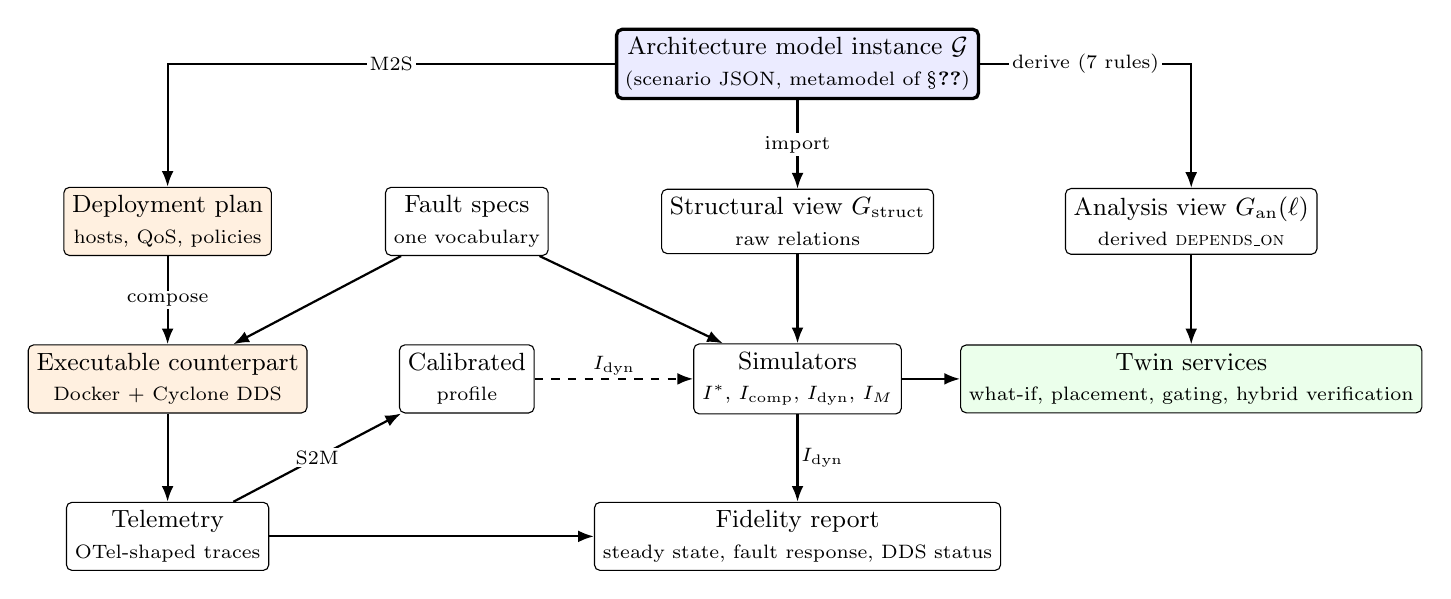
\begin{tikzpicture}[
  font=\small,
  art/.style={draw, rounded corners=2pt, align=center, minimum height=8mm, inner sep=3pt, fill=white},
  mdl/.style={art, fill=blue!8, very thick},
  phys/.style={art, fill=orange!12},
  svc/.style={art, fill=green!8},
  trans/.style={-{Latex[length=2mm]}, thick},
  dtrans/.style={-{Latex[length=2mm]}, thick, dashed},
  lbl/.style={font=\scriptsize, align=center, fill=white, inner sep=1pt}
]
\node[mdl] (m) at (0,0) {Architecture model instance $\mathcal{G}$\\ \scriptsize(scenario JSON, metamodel of \S\ref{sec:metamodel})};
\node[phys] (plan) at (-8,-2) {Deployment plan\\ \scriptsize hosts, QoS, policies};
\node[art]  (faults) at (-4.2,-2) {Fault specs\\ \scriptsize one vocabulary};
\node[art]  (gs) at (0,-2) {Structural view $\Gs$\\ \scriptsize raw relations};
\node[art]  (ga) at (5,-2) {Analysis view $\Ga(\ell)$\\ \scriptsize derived \textsc{depends\_on}};
\node[phys] (tb) at (-8,-4) {Executable counterpart\\ \scriptsize Docker + Cyclone DDS};
\node[art]  (cal) at (-4.2,-4) {Calibrated\\ \scriptsize profile};
\node[art]  (sim) at (0,-4) {Simulators\\ \scriptsize $I^*$, $\Icomp$, $\Idyn$, $I_M$};
\node[svc]  (svc) at (5,-4) {Twin services\\ \scriptsize what-if, placement, gating, hybrid verification};
\node[art]  (tel) at (-8,-6) {Telemetry\\ \scriptsize OTel-shaped traces};
\node[art]  (fid) at (0,-6) {Fidelity report\\ \scriptsize steady state, fault response, DDS status};

\draw[trans] (m) -| node[lbl, pos=0.25]{M2S} (plan);
\draw[trans] (m) -- node[lbl]{import} (gs);
\draw[trans] (m) -| node[lbl, pos=0.25]{derive (7 rules)} (ga);
\draw[trans] (plan) -- node[lbl]{compose} (tb);
\draw[trans] (faults) -- (tb);
\draw[trans] (faults) -- (sim);
\draw[trans] (gs) -- (sim);
\draw[trans] (ga) -- (svc);
\draw[trans] (sim) -- (svc);
\draw[trans] (tb) -- (tel);
\draw[trans] (tel) -- node[lbl]{S2M} (cal);
\draw[dtrans] (cal) -- node[lbl, above]{$\Idyn$} (sim);
\draw[trans] (tel) -- (fid);
\draw[trans] (sim) -- node[lbl, right]{$\Idyn$} (fid);
\end{tikzpicture}}
\caption{Artefacts and transformations of the architectural digital twin. Blue: single model instance. Orange: executable counterpart playing the physical role. Green: engineering services, including closed-batch hybrid verification. Calibration and fidelity comparison apply to $\Idyn$; one fault vocabulary drives both simulation and the counterpart.}
\label{fig:architecture}
\end{figure}

\subsection{Metamodel: one instance, two views}
\label{sec:metamodel}

\begin{definition}[Architecture model]
An architecture model is a typed, weighted, directed multigraph $\mathcal{G} = (V, E, \tau_V, \tau_E, w_V, w_E)$ with weights $w_V, w_E \in [0.01, 1]$, vertex types
\[\tau_V : V \to \{\textsf{Application}, \textsf{Library}, \textsf{Topic}, \textsf{Broker}, \textsf{Node}, \textsf{NetworkDevice}\},\]
and edges $E = E_s \cup E_d$ partitioned into derived edges $\tau_E(E_d) = \{\textsc{depends\_on}\}$ and structural relations
\[\tau_E(E_s) \subseteq \{\textsc{publishes\_to}, \textsc{subscribes\_to}, \textsc{routes}, \textsc{runs\_on}, \textsc{connects\_to}, \textsc{uses}\}.\]
Topics carry QoS contracts (reliability, durability, history depth, deadline, priority, payload size, rate); hosts carry capacities; undirected \textsc{connects\_to} edges (modelled as symmetric pairs) carry link capacity and latency.
\end{definition}

Each instance exposes two views: the \textbf{structural view} $\Gs = (V, E_s)$ and the \textbf{analysis view} $\Ga(\ell)$, which holds \textsc{depends\_on} edges derived by seven rules (extending \citealp{yigit2025graph}) and filtered by layer $\ell \in \{\text{app}, \text{infra}, \text{mw}, \text{system}\}$:
\begin{enumerate}[leftmargin=*,nosep]
  \item a subscriber depends on its topics' publishers (including through library chains);
  \item an application depends on the broker routing its topics;
  \item a subscriber's host depends on the publisher's host (Rule~1 lifted);
  \item an application's host depends on the routing broker's host (Rule~2 lifted);
  \item an application depends on the libraries it uses;
  \item brokers on the same host share fate;
  \item a host depends on network devices separating it from a host it depends on.
\end{enumerate}
Rules~1--2 combine shared topics by probabilistic union and Rules~3--4 by worst-case lift~\citep{sag-software}. Crucially, \emph{analysis consumes $\Ga$ while simulation consumes $\Gs$ only} (R3). Simulators that need dependency arcs (change propagation and library-chain fault injection) re-derive them independently from $\Gs$, guarded against drift by CI invariants (\S\ref{sec:consistency}).

\subsection{Twin services}
\label{sec:services}

The twin provides four engineering services, each graded independently of the model that produced the proposal:
\begin{description}[leftmargin=1em,style=nextline,nosep]
  \item[What-if failure analysis.] Four simulators on $\Gs$~\citep{yigit2026jss} serve as behavioural models: cascade reachability ($I^*$), multi-layer composite ($\Icomp$), discrete-event SimPy queue-flow delivery loss ($\Idyn$, \citealp{team2020simpy}) and upstream change ripple ($I_M$). Opt-in $\Idyn$ extensions (queued physical links, latency-SLA degradation and LHS/Sobol uncertainty sweeps) are detailed in the online supplement~\citep{sag-software}.
  \item[Placement verification.] An exact optimiser proposes placements under host capacities, failure domains and replica counts; proposals are re-scored on a held-out replica-aware failure simulation and accepted only above a measured noise bar.
  \item[Change gating.] Rebuilds the twin on candidate changes and blocks only on \emph{newly introduced} structural defects (e.g.\ new single points of failure or cycles); impact rankings remain advisory rather than blocking~\citep{yigit2026jss}.
  \item[Hybrid two-tiered verification.] The CLI entry point \texttt{saag-simulate hybrid-verify} chains one fault-free baseline and calibration (Step~0), calibrated Tier-1 $\Idyn$ screening with order-$k$ references (Step~1), deterministic shortlisting of top-$K$ targets, disagreements and negative controls (Step~2), and targeted Tier-2 counterpart probing with crash and gray failures (Step~3), emitting machine-readable caveats and an operational health summary.
\end{description}

\subsection{Maturity: what is built and what is designed}
\label{sec:maturity}

Table~\ref{tab:maturity} adapts \citet{kritzinger2018digital} by inserting a \emph{generated counterpart} rung. Present tense throughout describes built capabilities; designed capabilities use requirements voice in \S\ref{sec:livetwin}. Even though M2S and S2M are automated, an engineer closes the loop per run and the counterpart is an emulation, satisfying \citet{wright2020tell} only for \emph{middleware, timing and transport behaviour under declared application behaviour}.

\begin{table}[t]
\centering
\caption{Maturity of the architectural twin on the ladder of \citet{kritzinger2018digital}. ``Counterpart'' is the emulated system (\S\ref{sec:m2s}) or, at the twin level, a deployed system.}
\label{tab:maturity}
\small
\begin{tabularx}{\textwidth}{@{}l Y Y l@{}}
\toprule
Level & Model $\to$ counterpart & Counterpart $\to$ model & Status \\
\midrule
Digital model & Model authored/extracted; analysis and simulation run on it. & None. & built \\
Generated counterpart & Model compiled automatically into Docker + DDS deployment and chaos plan (\S\ref{sec:m2s}). & None. & built \\
Digital shadow (batch) & As above. & Automated trace calibration and fidelity reports (\S\S\ref{sec:s2m}--\ref{sec:fidelity}) via standalone or \texttt{hybrid-verify} runs; batch drift detection, EMA re-calibration and residual feedback evaluated on perturbed Docker counterparts (\S\ref{sec:evaluation}). Invoked per run by an engineer. & built \\
Digital twin & Engineer-approved decisions pushed to deployed system. & Continuous ingestion; topology-drift graph diffing and repair proposals (\S\ref{sec:livetwin}). & designed \\
\bottomrule
\end{tabularx}
\end{table}

\section{Model to System: Generating the Executable Counterpart}
\label{sec:m2s}

The twin needs a physical side before the real system exists (R4). We generate one: the model instance is compiled into a deployment in which every modelled host is a Docker container and every modelled application and broker is a process that speaks real DDS. The physical side is therefore whatever the model says it is, which is the source both of its value and of its limits. This section describes the transformation in three stages (Figure~\ref{fig:m2s}) and then the trace links that make its output auditable.

\begin{figure}[t]
\centering
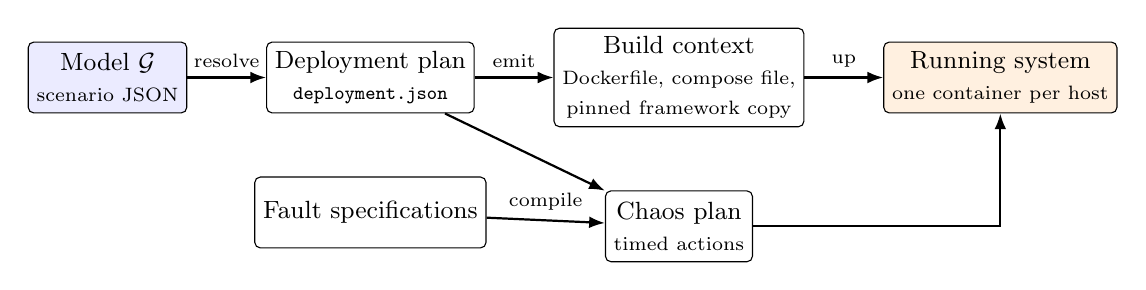
\begin{tikzpicture}[font=\small,
  box/.style={draw, rounded corners=2pt, align=center, minimum height=9mm, inner sep=3pt},
  ar/.style={-{Latex[length=2mm]}, thick}]
\node[box, fill=blue!8] (g) {Model $\mathcal{G}$\\\scriptsize scenario JSON};
\node[box, right=10mm of g] (p) {Deployment plan\\\scriptsize \texttt{deployment.json}};
\node[box, right=10mm of p] (c) {Build context\\\scriptsize Dockerfile, compose file,\\\scriptsize pinned framework copy};
\node[box, right=10mm of c, fill=orange!12] (r) {Running system\\\scriptsize one container per host};
\node[box, below=8mm of p] (f) {Fault specifications};
\node[box, below=8mm of c] (a) {Chaos plan\\\scriptsize timed actions};
\draw[ar] (g) -- node[above,font=\scriptsize]{resolve} (p);
\draw[ar] (p) -- node[above,font=\scriptsize]{emit} (c);
\draw[ar] (c) -- node[above,font=\scriptsize]{up} (r);
\draw[ar] (f) -- node[above,font=\scriptsize]{compile} (a);
\draw[ar] (p) -- (a);
\draw[ar] (a) -| (r);
\end{tikzpicture}
\caption{The model-to-system transformation. Everything an agent needs is resolved once into the plan, so all containers agree on it. The chaos plan is compiled from the same fault specifications the simulators consume.}
\label{fig:m2s}
\end{figure}

\subsection{Stage 1: resolving a deployment plan}

The first stage resolves the model into a \emph{deployment plan}: a self-contained document from which every per-host agent reads its configuration, so that no agent re-interprets the model on its own. The plan fixes four groups of facts.

\begin{itemize}[leftmargin=*]
  \item \textbf{Topics.} The plan records each topic's rate, QoS contract, payload size, publishers and routing brokers.
  \item \textbf{Applications.} The plan records each application's inputs and outputs, its hosts and its trigger policy. The trigger policy says when an application emits: on its own period, or only when its inputs are fresh. Policies are taken from the model, or resolved by the same function the simulator's reactive behaviour model uses. With \emph{open-loop} planning, every application emits on schedule, which is the assumption of the published queue-flow simulator. The plan also records a staleness window for each required input and a mean service time. That time is set so that each application station runs at a declared target utilisation, 0.65 by default, of its input load.
  \item \textbf{Brokers.} The plan records the routed topics and service times of each broker.
  \item \textbf{Hosts.} The plan records the residents of each host. An application with several \textsc{runs\_on} edges gets one instance per host, and a component with none is placed on a default host. Under CPU-bound emulation, the plan also records each container's CPU cap, which is the model's declared core count, or else one core per resident station.
\end{itemize}

The plan is the only place where model semantics become run-time configuration. It is produced by the same functions that configure the simulator. A disagreement between twin and counterpart therefore points at timing and transport, not at a second, divergent reading of the model.

\subsection{Stage 2: mapping model concepts to DDS}

Some model concepts have no direct DDS counterpart. Three mappings deserve discussion.

\paragraph{QoS.} Model-level QoS maps onto DDS policies as shown in Table~\ref{tab:qosmap}. The mapping is kept as plain data, separate from the middleware binding. It can therefore be unit-tested without DDS installed, and it can be reviewed as a modelling decision rather than buried in code.

\begin{table}[t]
\centering
\caption{Mapping from model-level topic QoS to DDS policies in the generated counterpart.}
\label{tab:qosmap}
\small
\begin{tabular}{@{}ll@{}}
\toprule
Model attribute & DDS policy \\
\midrule
reliability & \textsc{Reliable} (max.\ blocking 100\,ms) / \textsc{BestEffort} \\
durability & \textsc{Volatile} / \textsc{TransientLocal} / \textsc{Transient} / \textsc{Persistent} \\
history depth & \textsc{KeepLast}($d$), with $d=100$ when absent \\
deadline & \textsc{Deadline}, only when declared \\
transport priority & \textsc{TransportPriority} (low 0 \ldots\ critical 3) \\
payload size & zero-filled payload of that size (optional) \\
--- & \textsc{Liveliness} \textsc{Automatic}, lease 1\,s (plan-wide) \\
\bottomrule
\end{tabular}
\end{table}

\paragraph{Brokers on a brokerless middleware.} DDS is peer-to-peer, but the metamodel has a \textsf{Broker} type with \textsc{routes} edges, because systems built on Kafka, MQTT or enterprise buses depend on brokers. Dropping brokers would make an entire class of modelled failures unobservable. Each broker is therefore emulated as a relay process. Writers publish into an \emph{ingress} partition, and the routing broker republishes into the \emph{egress} partition that readers use. When several brokers route a topic, the lowest-identifier broker whose heartbeat is still within its lease (1\,s) is active. A broker outage thus becomes a real loss of delivery, with real failover, on a middleware that has no brokers of its own. The relays' own DDS endpoints exist only on the counterpart, so they are excluded from status comparisons and counted separately (\S\ref{sec:fidelity}).

\paragraph{Replicas.} An application with several hosts runs one instance per host. The lowest-identifier live instance is active. The others are warm standbys: they track input freshness but neither serve nor emit, and they take over after a 1\,s lease. This is the counterpart of the simulator's replica-aware semantics, in which a host outage moves an application rather than killing it. It is also what makes the twin's placement-verification service (\S\ref{sec:services}) testable on the counterpart.

The stub applications behave like the simulator's application model, in real time:
\begin{itemize}[leftmargin=*,nosep]
  \item one publisher thread per output topic;
  \item a single worker thread serving all inputs, which is the simulator's shared station;
  \item bounded receive queues with the model's overflow policy;
  \item deadline checks on end-to-end latency.
\end{itemize}
Samples are taken by a poller thread blocked on a DDS WaitSet, never by middleware listener callbacks. We learned this the hard way: a Python listener runs on the middleware's receive thread while that thread holds the reader's lock and waits for the interpreter lock, which stalls reception under load. Such details are invisible in the model. Yet they decide whether the counterpart measures the middleware or the emulation harness, which is why we report them.

\subsection{Stage 3: emitting a build context}

The plan is emitted as a build context: a Dockerfile, a compose file with one container per host on a shared bridge network (so DDS discovery works), and a copy of the framework itself. Copying the framework pins the image to the exact code that wrote the plan, so a counterpart cannot silently run a newer emulator than the one the plan was written for. The middleware version is pinned (Cyclone DDS 11.0.1) and changed only deliberately. Containers receive the \texttt{NET\_ADMIN} capability so that the chaos layer can partition them.

Two emulation options are opt-in at build time:
\begin{itemize}[leftmargin=*]
  \item \textbf{CPU-bound service.} Each stub burns its service time on the CPU instead of sleeping, and each container is capped at its plan CPU count. Co-located applications then really compete for a host, as they do in the simulator's host model. The build refuses to run when the requested utilisation exceeds the machine's cores, so an overloaded emulator is never mistaken for an overloaded system.
  \item \textbf{Payload carrying.} Each topic's declared payload size is put on the wire. Serialisation costs about 12\,ns per byte in our setup, about 0.4\,ms for 32\,KiB.
\end{itemize}

\subsection{One fault vocabulary, two back-ends}
\label{sec:faults}

Faults are specified once, as a list of fault specifications. Each one gives a target, a mode, a start time and a duration; link flaps also carry the parameters of a Gilbert--Elliott schedule. The same list is consumed by the simulators and by the counterpart's chaos compiler (Table~\ref{tab:chaos}). For a link flap, both back-ends draw the bad periods from the same seeded schedule.

\begin{table}[t]
\centering
\caption{Compilation of fault specifications into actions on the counterpart. Application-level faults reach a process inside a container through a control file that the host agent polls every 0.1\,s.}
\label{tab:chaos}
\small
\begin{tabularx}{\textwidth}{@{}l Y@{}}
\toprule
Fault (target, mode) & Counterpart action \\
\midrule
Host crash & \texttt{docker kill} of the host's container \\
Host transient crash & \texttt{docker kill}, later \texttt{docker start}; residents restart fresh, telemetry is appended \\
Host freeze & \texttt{docker pause} / \texttt{unpause} \\
Host slowdown & slowdown control file for every resident \\
Application or broker crash, transient crash, freeze, slowdown, omission, babbling & control file read by the agent, reset when the fault ends \\
Link flap & a \emph{partition} during each bad period: blocked containers drop ingress traffic (unicast and multicast) from each other's addresses with \texttt{tc}, so DDS discovery and liveliness see the cut \\
Network-device crash (with network gating) & a partition of every host pair that \textsc{connects\_to} no longer connects \\
Buffer leak, redelivery storm & reported as \emph{unsupported}, never silently skipped \\
\bottomrule
\end{tabularx}
\end{table}

\paragraph{Network gating.} Without network gating, a link flap blocks exactly the two hosts at its ends. With gating, the chaos compiler removes cut links and crashed hosts or devices from the \textsc{connects\_to} graph and blocks every host pair that is no longer connected. This is the same reachability rule the simulator applies, implemented once in a shared module. A model whose topology already separates some hosts is partitioned before traffic starts, so the counterpart cannot be more connected than its model.

Reporting unsupported faults is a small design decision that matters for a twin. Suppose a fault were silently dropped on one back-end. The fidelity report would then compare a faulted simulation with an unfaulted counterpart, and the twin would look either better or worse than it is.

\subsection{Trace links}
\label{sec:tracelinks}

Every artefact of a counterpart run can be traced to the model element that produced it:
\begin{itemize}[leftmargin=*]
  \item containers are named after modelled hosts;
  \item DDS topic names are derived from modelled topic identifiers;
  \item each telemetry event carries the identifier of the modelled component that emitted it and of the modelled topic involved;
  \item control files are named after the targeted component.
\end{itemize}
A run directory therefore contains the plan, the build context, the per-host telemetry, the run metadata, the calibrated profile and the fidelity report. Any fidelity finding can be followed back to a model element and forward to the container that exhibited it. This auditability is what the model-driven twin literature asks for when it calls for traceable synchronisation between twin and system~\citep{bordeleau2020towards}. Here it is a by-product of generating, rather than hand-building, the counterpart.

\section{System to Model: Telemetry and Calibration}
\label{sec:s2m}

A pre-deployment model has to guess the runtime parameters that drive its behavioural simulation:
\begin{itemize}[leftmargin=*,nosep]
  \item how often each topic is really published;
  \item how long each application takes to serve a message;
  \item whether an application emits on its own schedule or only when its inputs are fresh.
\end{itemize}
After deployment, or on the counterpart, these can be measured. The system-to-model transformation turns a trace into a \emph{calibrated profile} that overrides the declared values in the queue-flow simulator (R5). Its design rests on two principles. First, every fitted value records where it came from. Second, the calibrator abstains rather than guesses when the trace does not determine a parameter.

\subsection{Trace schema}

Telemetry is a stream of JSON-lines events shaped like OpenTelemetry log records. Every event has a timestamp on a clock shared by all agents, an event name, and attributes that use OpenTelemetry's messaging conventions where they exist (\texttt{service.name}, \texttt{messaging.\allowbreak destination.\allowbreak name}, \texttt{messaging.\allowbreak message.\allowbreak id}). Six event kinds are defined:
\begin{itemize}[leftmargin=*,nosep]
  \item \emph{publish}, for an emission;
  \item \emph{deliver}, for a sample processed within its deadline, with latency and service time;
  \item \emph{deadline miss}, for a sample that was processed and then dropped as late; it carries its service time too;
  \item \emph{drop}, for a queue overflow;
  \item \emph{state}, for a component state change such as crash, recovery or replica takeover;
  \item \emph{status}, for periodic DDS status counts.
\end{itemize}

The queue-flow simulator writes the \emph{same} schema when asked to record events. This is the single most useful decision in the system-to-model path. Calibration and fidelity comparison are written once and applied to simulated and observed traces alike. A difference between the two can then never be an artefact of two parsers.

\subsection{The calibrator}

The calibrator fits three groups of parameters on the post-warm-up window of a trace: topic rates and service-time distributions on fault-free steady state, and trigger policies whenever the trace contains discriminating input outages.

\paragraph{Topic rates.} The fitted rate of a topic is its emissions per second, counted over all of its publishers.

\paragraph{Service-time distributions.} For each application the calibrator records the mean and coefficient of variation of its measured service times. It reports an exponential family when the CV lies in $[0.7, 1.3]$ and a lognormal family otherwise, and it fits only when at least five samples exist. Service times are taken from delivered samples \emph{and} from samples dropped as late. A late sample was still served, and fitting only the on-time survivors biases the mean low. On the ATM scenario, this bias put one application's mean 45\% low before the schema carried service times on deadline misses.

\paragraph{Trigger policies.} An application with inputs either emits periodically regardless of its inputs (\emph{periodic}), stops only when all inputs are stale (\emph{any-of}), or stops as soon as one input is stale (\emph{all-of}). The calibrator infers which by splitting time into three input states: all fresh, some stale, and all stale. In each state it compares the application's realised emission rate with its active rate. A state counts as evidence only if it lasted long enough to expect at least three emissions, and emission shares in an ambiguous middle band count as no evidence either way. If the trace never puts the application through a discriminating outage, the calibrator abstains. For a single-input application, the two reactive policies coincide, and the calibrator reports the simpler one.

\paragraph{What the calibrator refuses to write.} The behavioural profile also has slots used by other simulators. One is a per-edge \emph{failure correlation}, which is a cascade-propagation probability in the multi-layer failure simulator. Another is a starvation tolerance. A measured message-drop rate looks superficially like the former, but it is a different quantity, and no trace event measures the latter. The calibrator writes neither. In a twin, a model slot filled with a plausible but semantically wrong measurement is worse than an empty slot, because it is indistinguishable from a real calibration.

\paragraph{Closing the calibration loop into Tier-1 sweeps.} Both single-fault fidelity comparisons and full-system Tier-1 runtime sweeps (\texttt{runtime-sweep --profile}) consume the serialised \texttt{profile.json} via \texttt{telemetry\_profile}. The resulting runtime-label artefact records \texttt{calibrated: true} and \texttt{calibration\_source} while keeping its settings JSON-serialisable, so calibrated Tier-1 screening and uncalibrated declared sweeps remain cleanly distinguishable downstream.

\subsection{Identifiability: what telemetry can and cannot recover}
\label{sec:identifiability}

Calibration is only useful if it recovers the right values. To test this, we simulated the 74-component ATM scenario with \emph{known} parameters under the runtime-label settings, calibrated the resulting trace, and compared the fitted values with the known ones (Table~\ref{tab:identifiability}). The experiment is an automated test in the framework, so it is re-run on every change to the calibrator.

\begin{table}[t]
\centering
\caption{Parameter recovery on the ATM scenario: simulate with known parameters, calibrate the trace, compare (60\,s trace).}
\label{tab:identifiability}
\small
\begin{tabularx}{\textwidth}{@{}l l Y@{}}
\toprule
Parameter & Recovered? & Evidence \\
\midrule
Topic rates & yes & median relative error 3\% \\
Service mean and CV & yes & median relative error 1\%; every application within sampling noise (at most 3.6 standard errors, 30 applications); a uniform distribution is returned as lognormal with its true CV of 0.115 \\
Trigger policy & yes, when observable & 16--17 of the 17 applications with inputs and outputs receive an answer, and every answer is correct, for true staleness windows of 2, 3 or 6 periods (the calibrator assumes 3) \\
Staleness window & no & no estimator; the trace does not determine it \\
Burst ratio & no & no estimator; the trace does not determine it \\
\bottomrule
\end{tabularx}
\end{table}

The negative rows are results, not omissions. They tell the twin's users that post-deployment data cannot narrow the plausible range of two behavioural parameters. Any conclusion sensitive to those parameters must keep carrying their uncertainty after deployment. Applications that never experienced a partial input outage receive no policy, which is correct behaviour rather than a gap.

An identifiability table of this kind is cheap to produce once the simulator and the counterpart share a trace schema, and we recommend it as a standard artefact for calibrated twins. It separates three kinds of parameter:
\begin{itemize}[leftmargin=*,nosep]
  \item parameters that data can pin down;
  \item parameters that data can pin down only under particular operating conditions (here, trigger policies need an outage);
  \item parameters that data cannot pin down at all.
\end{itemize}
Without such a table, a calibrated twin silently presents all three as equally ``calibrated''.

The identifiability test uses a simulated trace as ground truth, so it checks the estimators, not the counterpart. Applying the calibrator to counterpart traces, and asking whether calibration improves fidelity, is hypothesis H5 of the fidelity study (\S\ref{sec:protocol}).

\section{Fidelity Assessment}
\label{sec:fidelity}

Fidelity is among the least operationalised characteristics of digital twins~\citep{jones2020characterising}. We define three comparison dimensions (\S\ref{sec:dimensions}), separate independent evidence from shared construction (\S\ref{sec:independence}), and freeze our confirmatory analysis in a pre-registered protocol (\S\ref{sec:protocol}).

\subsection{Fidelity dimensions and feedback diagnostics}
\label{sec:dimensions}

Every fidelity report compares one simulated trace ($\Idyn$) against one observed trace in the shared schema of \S\ref{sec:s2m}, never gating builds (R6):
\begin{itemize}[leftmargin=*,nosep]
  \item \textbf{Steady state:} Per-element errors against default tolerances (5\% topic publication rate, 10\% reader delivery rate, 25\%/35\% p50/p95 latency, 0.05 absolute deadline-miss share; supplement Table~S3~\citealp{sag-software}).
  \item \textbf{Fault response:} Observed impact $\Iobs(v)$ mirrors $\Idyn$'s definition (pre-fault minus post-fault delivery rate over surviving readers, matching engine $\Idyn$ within 0.0002 on ATM). We compare impact rankings via Spearman's $\rho$ (with top-$K$ Jaccard also computed in operational triage reports) and per-fault stalled reader sets via Jaccard index $J$.
  \item \textbf{Middleware status:} Compares entities with non-zero DDS counters (liveliness alive/not-alive, offered/requested deadline misses, lost/rejected/cache-replaced samples), excluding broker-relay endpoints.
\end{itemize}
An operational health evaluator also aggregates per-entity states into ISO/IEC~25019 quality-in-use indices~\citep{iso25019}, and two advisory diagnostics---\texttt{detect\_drift} and \texttt{diagnose\_\allowbreak fault\_\allowbreak residuals}---feed fidelity breaches back to calibration (\S\ref{sec:evaluation}).

\subsection{Independence analysis: what the counterpart can show}
\label{sec:independence}

Because the counterpart is generated from the same model as the simulators, reporting shared-construction agreement as fidelity would be circular~\citep{sargent2013verification}. Table~\ref{tab:independence} classifies every counterpart element before any comparison. \emph{The strongest attainable conclusion concerns timing, middleware and transport fidelity on an emulated system under declared behaviour---never real production application logic.} To keep these boundaries machine-readable, \texttt{hybrid-verify} emits structured \texttt{caveats} in every report (flagging reactive circularity, rate-scaled latency distortion, DDS rediscovery lag, and skipped unsupported probes).

\begin{table}[t]
\centering
\caption{Independence analysis of the generated counterpart. Only agreement on the independent row counts as fidelity evidence.}
\label{tab:independence}
\small
\begin{tabularx}{\textwidth}{@{}Y l Y@{}}
\toprule
Counterpart part & Independent? & Consequence \\
\midrule
DDS delivery, discovery and liveliness; OS scheduling; real elapsed time; container kills and network partitions & yes & what fidelity results can speak to \\
Topic rates, mean service times, queue bounds, failover rule, placement & no (same plan) & agreement is not evidence \\
Trigger policies (reactive behaviour) & no (shared function) & reactive simulator vs.\ reactive counterpart is circular \\
Late-sample handling & no (configured rule) & engine late-drop mode is never treated as truth \\
Application logic & no (stubs) & no result covers real application behaviour \\
\bottomrule
\end{tabularx}
\end{table}

\subsection{A pre-registered fidelity study}
\label{sec:protocol}

To prevent post-hoc metric or scenario selection, we froze the confirmatory study protocol on 16 November 2026 (commit \texttt{9f84aad9}; simulator arms and analysis executed on tag \texttt{fidelity-study-arms-code}) before computing any simulator--counterpart comparison~\citep{sag-software}. Only capacity and noise pilots ran before freezing. Full exclusion, rerun and amendment rules are archived in the repository supplement~\citep{sag-software}.

\paragraph{Population, capacity gate and amendments.} The unit of analysis is the \emph{scenario} (avoiding pseudo-replication across components or seeds). Twelve candidate scenarios (eleven generated domains plus ATM) faced a fault-free capacity gate (rate error $\le 5\%$, container CPU p95 $\le 80\%$, rate-scaling factor $\kappa \ge 0.2$ from pilot capacity $B_h = 3{,}033$\,msg/s). Nine passed at full rate ($\kappa = 1$), so latency counts on every included scenario; \texttt{av} (CPU gate), \texttt{enterprise} (peer-discovery/rate gate) and \texttt{financial\_trading} ($\kappa < 0.2$) were excluded. Two blinded amendments were registered before any simulator arm ran: Amendment~1 judged standby-only hosts (\texttt{industrial\_scada}'s \texttt{N4}) by container liveness instead of log recency; Amendment~2 withdrew \texttt{industrial\_scada} for compute cost ($\approx 400$ re-runs), yielding $n = 8$.

\paragraph{Conditions, arms and hypotheses.} The confirmatory condition (\textbf{O-open}) makes all applications periodic to avoid trigger-policy circularity (Table~\ref{tab:independence}); \textbf{O-react} is descriptive only. Seven arms are compared against $\Iobs$ (three repetitions per target): \textbf{S0} (published queue-flow engine), \textbf{S1} (S0 + DDS deadline semantics), \textbf{S2} (current model: S1 + host stations, per-process RNG, replica awareness), \textbf{S3} (S2 calibrated from a disjoint fault-free run, respecting R5 vs.\ R6), \textbf{S4} (reactive S2, O-react only), \textbf{R} (closed-form first-order rate $\times$ readership formula, no simulation), and \textbf{N} (shuffled-label instrument check, must lie within $\pm 0.10$).

Primary hypothesis \textbf{H1} tests whether S2 ranks publishing applications closer to $\Iobs$ than S0 under O-open (one-sided exact Wilcoxon~\citealp{wilcoxon1945individual}, $\alpha = 0.05$, Hodges--Lehmann effect size + 95\% CI, TOST equivalence against $\delta = 0.05$ fixed from the noise pilot), mapped by a pre-fixed decision table onto \emph{better}, \emph{equivalent}, \emph{inconclusive} or \emph{worse}. A Holm-corrected two-sided secondary family tests \textbf{H2} ($\rho(\mathrm{S0}) > 0.70$), \textbf{H3} (S2 vs.\ R), \textbf{H4} (S0 vs.\ R) and \textbf{H5} (S2 vs.\ S3 delivery error). Every per-scenario $\rho$ is paired with the counterpart's leave-one-repetition-out noise ceiling $C_s$ and a formal claim table stating what each outcome licenses.

\section{Evaluation}
\label{sec:evaluation}

We evaluate four research questions---one per challenge of \S\ref{sec:intro}: \textbf{RQ1} (semantic consistency across artefacts), \textbf{RQ2} (parameter calibration and batch drift), \textbf{RQ3} (fidelity to the counterpart and divergences) and \textbf{RQ4} (service and counterpart cost). Every result carries an explicit provenance tag: \textbf{[P]} (open-source prototype, regenerable from committed artefacts), \textbf{[S1]} (frozen pre-registered Study~1, commit \texttt{9f84aad9}) or \textbf{[S2]} (frozen pre-registered Study~2, commit \texttt{0bbe06af}). Full per-scenario matrices and test breakdowns are archived in the online supplement~\citep{sag-software}.

\subsection{Subjects}

Subjects come from the framework's byte-reproducible scenario corpus~\citep{sag-software}: the 74-component \texttt{atm} scenario, a five-member ATM scale family (29--444 components), eleven generated domain scenarios (including autonomous vehicles, IoT, healthcare, telecom RAN, microservices and industrial control), two pilot scenarios excluded from the study populations (\texttt{tiny\_system}: 4 hosts, 12 apps, 2 brokers; and an integration-hub pilot), and five real-world OSS architecture topologies (\texttt{autoware\_ros2}, \texttt{edgex}, \texttt{homeassistant}, \texttt{trainticket} and \texttt{cloud\_microservices}) included in Study~2 and the perturbed-counterpart evaluation.

\subsection{RQ1: Consistency across twin artefacts}
\label{sec:consistency}

Consistency is enforced by \textbf{103 automated pytest invariants} in CI [P] covering rule-by-rule \textsc{depends\_on} parity across Rules~1--7 (15 checks), in-memory vs.\ graph-database repository parity (3), substrate-import isolation (1), oracle-role separation (8), byte-identical scenario regeneration (21), M2S/chaos/in-process parity (34) and \texttt{hybrid-verify} contracts (21; full breakdown in supplement Table~S4~\citealp{sag-software}).

These invariants caught a real defect: the simulator's re-derivation originally implemented only 1 of 7 rules, silently zeroing $I_M$ for all scored components; the fix enforced full re-derivation and distinguished \emph{not measured} from zero. Conversely, one residual divergence remains documented as visible consistency debt: when a topic is reachable both directly and via a library, the in-memory repository double-counts its Rule~1 weight while the graph-database repository (and simulator) do not (0 pairs on \texttt{atm}, 64 on \texttt{microservices} with $\Delta w \le 0.248$, 139 on \texttt{av} with $\Delta w \le 0.374$ [P]).

\textbf{Answer to RQ1.} Automated CI invariants enforce rule-by-rule semantic agreement across all artefacts, caught a major historical bug, and keep residual edge-weight debt measured and visible.

\subsection{RQ2: Calibration identifiability and perturbed-counterpart recovery}

Table~\ref{tab:identifiability} (\S\ref{sec:identifiability}) shows that on ATM, calibration recovers topic rates within 3\% median error, application service means/CVs within 1\%, and trigger policies with 100\% accuracy when discriminating outages occur, while staleness windows and burstiness under periodic workloads remain non-identifiable; broker service times, \texttt{k\_of\_n:$K$} policies and bursty MMPP workloads are recovered in unit round trips [P]. On the unperturbed Study~1 counterpart, H5 is undecidable because uncalibrated S2 already has 0.000 per-reader delivery error in seven of eight scenarios (0.018 in the eighth, unchanged after calibration; HL $0.000$, Holm n.s.) [S1].

\paragraph{Perturbed-counterpart calibration and batch drift (Docker) [P].} To test calibration and R7 batch drift when pre-deployment guesses are actually misspecified, we perturbed the Docker + Cyclone DDS counterpart on \texttt{tiny\_system} (4 containers), \texttt{atm} (8 containers) and \texttt{realworld\_\allowbreak autoware\_\allowbreak ros2} (6 containers)---shifting 40\% of topic rates by $+50\% / -35\%$ and doubling service times on the busiest host while keeping the twin's prior at declared values (40\,s runs, 5\,s warm-up, 3 repetitions, calibration from a disjoint trace; supplement Table~S6~\citealp{sag-software}):
\begin{itemize}[leftmargin=*,nosep]
  \item \emph{Batch calibration (S2 $\to$ S3):} Cuts median delivery error by 77\% on \texttt{tiny\_system} ($0.277 \to 0.064$), 96\% on \texttt{atm} ($0.053 \to 0.002$) and 87\% on \texttt{realworld\_\allowbreak autoware\_\allowbreak ros2} ($0.284 \to 0.036$), and lowers p50/p95 latency error by 10--63\% across all three topologies (e.g.\ \texttt{realworld\_\allowbreak autoware\_\allowbreak ros2} p95: $0.620 \to 0.228$).
  \item \emph{Incremental EMA (\texttt{update\_profile}, $\alpha = 0.5$):} Delivery error converges monotonically across three rolling windows on every topology (\texttt{tiny\_system}: $0.161 \to 0.091 \to 0.087$; \texttt{atm}: $0.059 \to 0.040 \to 0.029$; \texttt{realworld\_\allowbreak autoware\_\allowbreak ros2}: $0.118 \to 0.062 \to 0.038$).
  \item \emph{Drift detection and residual feedback:} \texttt{detect\_drift} achieves 1.00 TP (shifted-topic recall 0.73--1.00), but also flags unperturbed baselines ($\text{FP} = 1.00$) despite 0.28\% median baseline delivery error (0.28--2.86\% across the three topologies) because single-machine p50 latency exceeds 25\% on $>20\%$ of topics---showing that rate/delivery and latency drift require separate thresholds. Under a behavioural shift (one app changed from \emph{periodic} to \emph{all-of}), \texttt{diagnose\_fault\_residuals} correctly infers \emph{all-of} on \texttt{tiny\_system} (\texttt{A11}) and \texttt{realworld\_\allowbreak autoware\_\allowbreak ros2} (\texttt{A10}), and \emph{any-of} on \texttt{atm} (\texttt{A1}).
\end{itemize}

\textbf{Answer to RQ2.} Telemetry recovers rates, service times and observable trigger policies; under real parameter misspecification on Docker + DDS counterparts, batch calibration and rolling EMA cut delivery error by 77--96\% [P] and Study~2 confirmatorily validates delivery-error reduction across all 14 topologies (H2.3: median $0.082 \to 0.018$, HL $+0.096$, Holm $p = 0.00049$) [S2], whereas unperturbed Study~1 H5 has zero baseline error to reduce [S1]. Staleness windows and periodic-trace burstiness remain unidentifiable.

\subsection{RQ3: Fidelity of the simulators to the counterpart}
\label{sec:rq3}

\paragraph{Smoke test and a real middleware fidelity gap [P].} On \texttt{tiny\_system} in Docker (4 containers, 1\,Hz; supplement Table~S5~\citealp{sag-software}), fault-free, host-crash (\texttt{docker kill}) and broker-failover runs agree exactly on stalled readers ($J = 1.0$), exact DDS \texttt{liveliness\_\allowbreak alive\_\allowbreak count} across all 15 readers, and per-reader delivery within 5.9\% (p95 latency error 11--18\%, within 35\% tolerance; p50 14\% fault-free, 34--40\% under faults). Next, a 10\,s switch-crash partition on a two-host chain (with network gating and CPU-bound service matching 21.3\,ms vs.\ 22.5\,ms exponential median) stopped deliveries within 0.2\,s as simulated, but resumed \textbf{$\approx 6$\,s after the partition healed} whereas $\Idyn$ reconnects instantaneously: during partitions longer than the 1\,s participant lease, Cyclone DDS expires remote participants and must rediscover them. This independent-row finding (Table~\ref{tab:independence}) is invisible to any self-consistent simulator.

\paragraph{Pre-registered fidelity studies [S1] and [S2].} In Study~1 [S1], all 2,738 counterpart runs across $n = 8$ scenarios at $\kappa = 1$ passed validity on the first attempt (0.000 pre-fault rate error; peak CPU p95 38--62\%), simulator arms ran 10,950 times, and the instrument check passed ($\rho(\mathrm{N}) = 0.001$). In Study~2 [S2], all 14 topologies (13 at $\kappa = 1$, plus \texttt{cloud\_microservices} at $\kappa = 0.74$) completed cleanly ($\approx 18.0$\,h, $\approx 853$ Docker runs). Table~\ref{tab:study} summarises both studies (per-scenario matrices in supplement Tables~S7--S8~\citealp{sag-software}).

\begin{table}[t]
\centering
\caption{Pre-registered fidelity study results: Study~1 [S1] ($n = 8$, $\kappa = 1$, $\delta = 0.05$) and Study~2 [S2] ($n = 13$--$14$, independent rows). HL: Hodges--Lehmann median [95\% CI]. Holm-corrected secondary tests are two-sided.}
\label{tab:study}
\small
\begin{tabularx}{\textwidth}{@{}>{\raggedright\arraybackslash}p{0.26\textwidth} >{\raggedright\arraybackslash}Y >{\raggedright\arraybackslash}p{0.27\textwidth} >{\raggedright\arraybackslash}p{0.14\textwidth}@{}}
\toprule
Quantity & Statistic & Value & Decision \\
\midrule
\multicolumn{4}{@{}l}{\emph{Study~1 [S1] (commit \texttt{9f84aad9}, $n = 8$, O-open publishers)}} \\
H1: S2 vs.\ S0 (publishers) & HL [CI]; rank-biserial; $p_{\text{sup}}$; $p_{\text{TOST}}$ & $+0.014$ [$-0.002$, $0.094$]; 0.56; 0.098; 0.098$^{a}$ & \textbf{inconclusive} \\
H2--H5 (secondary, Holm) & H2 S0 vs.\ 0.70 ($p = 0.016$); H3 S2 vs.\ R ($0.84$); H4 S0 vs.\ R ($0.078$); H5 cal ($0.50$) & all arms \& R at ceiling ($\rho \approx 0.91$--$0.93$ vs.\ $C_s = 0.93$) & all n.s.\ (Holm) \\
Instrument check (arm N) & median $\rho_s(\mathrm{N})$ & 0.001 & within $\pm 0.10$ \\
\midrule
\multicolumn{4}{@{}l}{\emph{Study~2 [S2] (commit \texttt{0bbe06af}, $n = 13$--$14$, independent rows)}} \\
H2.1: p50 latency S0 $-$ S2 & $n = 13$ ($\kappa = 1$); HL [CI]; 1-sided $p$ & $+0.135$ [$+0.071$, $+0.225$]; $p = 0.00061$ & \textbf{better} \\
H2.2a: Infra $\rho - 0.85$ & $n = 14$; median $\rho$ (range); Holm $p$ & $0.979$ ($0.916$--$1.000$); $p_{\text{H}} = 0.00049$ & \textbf{significant} \\
H2.2b: Infra stall $J - 0.85$ & $n = 14$; median $J$; Holm $p$ & $1.000$ (all 14/14); $p_{\text{H}} = 0.00049$ & \textbf{significant} \\
H2.3: Perturbed cal S2 $-$ S3 & $n = 14$; HL [CI]; Holm $p$ & $+0.096$ [$+0.034$, $+0.182$]; $p_{\text{H}} = 0.00049$ & \textbf{significant} \\
H2.4: Omission vs.\ crash ref & $n = 14$; HL [CI]; raw $p$ & $+0.0003$ [$-0.0006$, $+0.0021$]; $p = 0.542$ & n.s.\ (Holm) \\
\bottomrule
\multicolumn{4}{@{}p{\textwidth}@{}}{\footnotesize $^{a}$Both $p$-values equal 25/256; a tie-aware permutation test gives $p_{\text{sup}} = 0.078$ (same decision).}\\
\end{tabularx}
\end{table}

\paragraph{Interpreting Study~1 and Study~2 together.} In Study~1, six scenarios differ by $|d_s| \le 0.02$, \texttt{logistics\_\allowbreak fleet} favours S0 by 0.020, and noisy \texttt{hub\_\allowbreak and\_\allowbreak spoke} ($C_s = 0.66$) favours S2 by 0.177, leaving H1 inconclusive. Every arm (S0--S3 and closed-form R) sits at the noise ceiling ($\rho \approx 0.91$--$0.93$ vs.\ $C_s = 0.93$): under O-open, a periodic publisher crash removes only direct-reader deliveries, which R computes directly from the shared plan (dependent rows of Table~\ref{tab:independence}). H2 clears 0.70 in 7/8 scenarios, but at $n = 8$ one loss floors two-sided $p$ at $0.016 > 0.0125$.

Study~2 confirms what Study~1's descriptive analyses suggested once the contrast moves to independent rows across 14 topologies (including five real-world OSS systems): (1)~host stations (S2) significantly lower steady-state p50 latency error from median 0.376 (S0) to 0.258 (11/13 wins; p95 $\le 0.30$ on all 13 full-rate scenarios, well inside the 35\% tolerance); (2)~on broker and host crashes (247 targets total), S2 ranks impact at median $\rho = 0.979$ (\texttt{autoware\_ros2} $= 1.000$) and achieves exact stall-set agreement ($J = 1.000$) on all 14 scenarios (after fixing Study~1's \texttt{healthcare} \texttt{A4} prime-second 59\,s silence-window artefact on \texttt{main}, while Study~1's frozen 0.28 stands); (3)~under parameter misspecification, S3 reduces delivery error on all 14/14 scenarios (median $0.082 \to 0.018$, and $0.161$--$0.334 \to 0.003$--$0.047$ on the five OSS topologies); and (4)~for top-3 publisher omissions ($p = 0.5$ over 10\,s, H2.4), small impact magnitudes leave both S2 and the crash reference with tiny absolute errors ($\approx 0.001$--$0.028$, with the clearest separation on \texttt{atm}: $0.0005$ vs.\ $0.020$) and no significant difference ($p = 0.542$). Study~1's descriptive DDS-status checks (40 faults: \texttt{liveliness\_alive\_count} and \texttt{offered\_deadline\_missed} $J = 0.98$; \texttt{requested\_deadline\_missed} 0.71; \texttt{cache\_\allowbreak replaced\_\allowbreak dropped\_\allowbreak samples} 0.50), sink controls ($I_{\mathrm{obs}} \in [0.002, 0.038]$) and O-react sensitivity ($\le 0.06$) are archived in the supplement~\citep{sag-software}.

\textbf{Answer to RQ3.} The counterpart confirms smoke-test stall sets and liveliness and exposes a 6\,s DDS post-partition rediscovery gap [P]. Study~1 shows open-loop publisher ranking is inconclusive and tied with closed-form R at the noise ceiling [S1]. Study~2 confirmatorily establishes that added model detail significantly improves steady-state latency (H2.1), reproduces broker/host crash rankings and exact stall sets (H2.2a/b), and makes S2M calibration effective under parameter misspecification (H2.3), while gray-failure omission error vs.\ a crash reference is n.s.\ (H2.4) [S2]. All counterpart evidence concerns $\Idyn$ alone.

\subsection{RQ4: Cost of the twin's services and counterpart}

Table~\ref{tab:cost} shows a five-order-of-magnitude cost ladder matching continuous-delivery stages: sub-second graph gating and graph simulators fit every commit; seconds-per-fault $\Idyn$ fits candidate screening; hybrid two-tiered verification scales with shortlist size rather than $|V|$---finishing in 54.2\,s in-process on \texttt{tiny\_system} and \textbf{107.4\,min measured} in Docker + DDS on \texttt{atm} for two fault probes ($\approx 48$--54\,min/probe, a 4--6$\times$ speedup over exhaustive sweeps, achieving 1.000 baseline health-state agreement across all 66 entities, Spearman $\rho = 1.000$ across the 5 primary \texttt{crash} targets [top-$K$ Jaccard 1.0], and exact rank agreement across the 3 non-host \texttt{omission} targets [\texttt{i\_flow} MAE 0.0008, stall-set $J = 1.0$; primary-only $\rho$ omitted at $n = 2$] while transparently skipping the 5 unsupported host-level omissions in \texttt{caveats}); and exhaustive counterpart sweeps ($\approx 18.0$\,h for Study~2; $\approx 56$\,h for Study~1; 10,950 simulator runs took 69\,min on 16 cores) fit periodic twin validation.

\begin{table}[t]
\centering
\caption{Cost ladder of twin services and counterpart: [P] except the last row [S1]/[S2]. Treat timings as orders of magnitude.}
\label{tab:cost}
\small
\begin{tabularx}{\textwidth}{@{}l Y l@{}}
\toprule
Artefact & Workload & Cost \\
\midrule
Change gate (analysis + checks) & ATM scale family, 29 / 74 / 148 / 296 / 444 components & 0.01--1.01\,s \\
Graph simulators ($I^*, \Icomp$) & 5-seed / exhaustive sweep, \texttt{atm} (74) / \texttt{av} (152) & 0.06--0.45\,s \\
Queue-flow simulator ($\Idyn$) & per fault (\texttt{atm}/\texttt{av}); 5-seed whole corpus & 1.5--4.3\,s (12.7\,CPU-h) \\
Hybrid verification (in-process) & \texttt{tiny\_system}: baseline + 17 Tier-1 $\times$ 2 seeds + 2 probes & 54.2\,s \\
Hybrid verification (Docker + DDS) & \texttt{atm}: baseline + 39 Tier-1 $\times$ 3 seeds + 8 targets $\times$ 3 reps $\times$ 2 probes & 107.4\,min ($\approx$48--54\,min/probe) \\
Counterpart (Docker + DDS) & single run; Study~2 (14 scenarios, $\approx 853$ runs) [S2]; Study~1 (8 scenarios, 2,738 runs) [S1] & $\approx$71\,s; $\approx$18.0\,h; $\approx$56\,h \\
\bottomrule
\end{tabularx}
\end{table}

\textbf{Answer to RQ4.} Matching each service to its rung on the five-order-of-magnitude cost ladder makes continuous architectural verification practical without running exhaustive container sweeps per change.

\section{Discussion}
\label{sec:discussion}

\subsection{Lessons for engineering architectural digital twins}

\begin{itemize}[leftmargin=*,nosep]
  \item \textbf{L1: Generate the physical stand-in; do not build it by hand.} Generating the counterpart from $\mathcal{G}$ ensures traceability (\S\ref{sec:tracelinks}), co-evolution, and enumerable shared assumptions for Table~\ref{tab:independence}.
  \item \textbf{L2: Share one trace schema across simulation and observation.} Writing calibration and fidelity once for both sides eliminates dual-parser drift; it is cheapest early and costliest to retrofit.
  \item \textbf{L3: Fidelity evidence requires an independence analysis.} Table~\ref{tab:independence} prevents mistaking shared-plan agreement (e.g.\ exact topic rates) for validation; the informative findings lie strictly in independent rows (stall sets, liveliness, partition rediscovery, latency).
  \item \textbf{L4: Calibrators must abstain and disclose unidentifiable parameters.} Table~\ref{tab:identifiability} keeps realistic-scale evidence separate from unit round trips and prevents presenting unobservable staleness windows or periodic burstiness as calibrated.
  \item \textbf{L5: Make consistency debt visible.} One model instance is not enough; executable CI parity checks catch silent re-derivation bugs while an explicit debt register documents unfixed divergences.
  \item \textbf{L6: Match each service to its rung on the cost ladder.} Sub-second gates per commit, queue-flow screening, $\approx$48--54\,min/probe Docker \texttt{hybrid-verify} for milestone triage, and machine-hour counterpart sweeps for periodic twin validation keep the twin viable in CI/CD.
\end{itemize}

\subsection{From digital shadow to live digital twin (R7)}
\label{sec:livetwin}

The twin reaches the batch-shadow level (Table~\ref{tab:maturity}), with batch parameter/behavioural drift detection (\texttt{detect\_drift}, \texttt{diagnose\_fault\_residuals}) and incremental EMA re-calibration (\texttt{update\_profile}) evaluated on perturbed Docker counterparts (\S\ref{sec:evaluation}). That evaluation showed that rate/delivery drift and latency drift must be thresholded separately because single-machine latency can exceed 25\% even when delivery agrees within 0.3\%. Three live-twin capabilities remain \emph{designed} (stated in requirements voice):
\begin{itemize}[leftmargin=*,nosep]
  \item \textbf{Continuous ingestion:} The twin shall ingest OTel-shaped telemetry continuously, tagged with project, platform and version.
  \item \textbf{Topology drift:} Observed (application, topic) relations differing from $\Gs$ shall produce a graph diff and an engineer-reviewed \emph{model-repair proposal}, never an automatic rewrite.
  \item \textbf{Engineer-in-the-loop actuation:} The twin shall push accepted re-placements or configuration changes only through engineers---never autonomous production actuation, which is inappropriate for mission-critical middleware.
\end{itemize}
Building calibration (R5) and measured fidelity with known noise (R6) before live drift detection (R7) is forced: drift is a fidelity breach on new data.

\subsection{Threats to validity}
\label{sec:threats}

\paragraph{Construct validity.} $\Iobs$ adopts $\Idyn$'s delivery-loss definition rather than latency; stall-set Jaccard ignores partial loss; and only $\Idyn$ (not $I^*$, $\Icomp$ or $I_M$) was compared against the counterpart.

\paragraph{Internal validity.} Shared plan parameters, trigger functions and late-sample rules are bounded by Table~\ref{tab:independence}. Single-machine Python emulation adds scheduling noise, guarded by the capacity gate, CPU logging and WaitSet polling, though large topologies like \texttt{enterprise} hit single-machine discovery limits (\S\ref{sec:protocol}).

\paragraph{External validity.} All counterparts use generated timing stubs over real Cyclone DDS instead of a physical production system; broker semantics are relay-emulated, Kafka/MQTT/ROS~2 back-ends are not built, and real application business logic is untested. While this is an intentional, explicitly bounded pre-deployment trade-off (\S\ref{sec:independence}), validating against an independently written DDS or ROS~2 application under the same fault vocabulary is the key next external step.

\paragraph{Conclusion validity.} In Study~1 ($n = 8$ after blinded Amendment~2), exact Wilcoxon floors prevented H2 from clearing Holm ($p = 0.016 > 0.0125$) and allowed noisy \texttt{hub\_and\_spoke} ($C_s = 0.66$) to decide H1; moreover, O-open publisher crashes exercised mainly the dependent rows of Table~\ref{tab:independence}, explaining the tie with closed-form R. Study~2 ($n = 13$--$14$) addressed both limitations directly on independent rows, reaching confirmatory significance on steady-state latency (H2.1), infrastructure crashes and stall sets (H2.2a/b) and perturbed calibration (H2.3), while gray-failure omission error (H2.4) remained non-significant.

\section{Conclusion}
\label{sec:conclusion}

We engineered an architectural digital twin for distributed publish--subscribe systems around one typed graph metamodel, deriving separated structural and analysis views guarded by 103 CI invariants (C1), compiling a runnable Docker + Cyclone DDS counterpart under a shared fault vocabulary (C2), calibrating $\Idyn$ over a shared OpenTelemetry-shaped trace schema with explicit identifiability limits (C3), and assessing fidelity through an independence analysis and frozen pre-registered study (C4). Claimed strictly at its built level---a digital model, generated counterpart and batch digital shadow---the twin recovers rates, service times and observable trigger policies, cuts delivery error by 77--96\% under Docker parameter perturbations with monotonic EMA convergence, matches smoke-test stall sets and DDS liveliness exactly, exposes a $\approx 6$\,s Cyclone DDS post-partition rediscovery gap, and fits CI/CD via a five-order-of-magnitude cost ladder (including measured Docker \texttt{hybrid-verify} on ATM).

Our two pre-registered studies yield complementary engineering lessons: Study~1 shows that under open-loop periodic behaviour, publisher-impact ranking saturates at the counterpart's noise ceiling and ties a closed-form first-order reference, proving that order-$k$ references must always be reported alongside simulators and confirmatory contrasts must target independent rows. Study~2 then confirms across 14 topologies (including five real-world OSS architectures) that added model detail significantly improves steady-state p50 latency (H2.1, $p = 0.00061$), reproduces broker/host crash rankings (H2.2a, $\rho = 0.979$) and exact stall sets (H2.2b, $J = 1.000$ on all 14/14), and makes S2M calibration effective under parameter misspecification (H2.3, 14/14 improved, Holm $p = 0.00049$). Turning this batch shadow into an engineer-in-the-loop live twin---adding continuous ingestion, topology-drift repair, and validation against an independently built DDS/ROS~2 system---is the natural next step.


\section*{Declarations}

\paragraph{Funding:} This work was supported in part by the Scientific and Technological Research Council of T\"urkiye (T\"UB\.ITAK), grant number [GRANT-NUMBER].

\paragraph{Competing Interests:} The authors declare that they have no competing financial or non-financial interests that are directly or indirectly related to the work submitted for publication.

\paragraph{Related Work by the Authors and Overlap Disclosure:} The following works by the same authors are related to this paper.
\begin{itemize}[leftmargin=*]
  \item \emph{Published.} \citet{yigit2025graph} introduced a reduced dependency-derivation method for publish--subscribe systems. This paper restates the extended metamodel in one condensed subsection (\S\ref{sec:metamodel}) and cites it.
  \item \emph{Under review.} A companion manuscript~\citep{yigit2026jss}, under review at the Journal of Systems and Software, develops the failure simulators as ranking oracles for learned criticality prediction. This paper uses those simulators as the twin's behavioural models, cites them, and reports none of that manuscript's results.
  \item \emph{Not in any other manuscript.} The model-to-system transformation and generated counterpart, the telemetry calibration and its identifiability analysis, the fidelity-assessment method and independence analysis, the smoke-test and partition results, the maturity analysis and the requirements condensation are reported here for the first time.
\end{itemize}
We disclose this so the editor can assess the overlap directly. \tbd{update if the companion manuscripts' status changes before submission}

\paragraph{Data Availability:} The framework, including the counterpart generator, calibrator and fidelity report, is open source~\citep{sag-software}. Scenario topologies, generator configurations, the fidelity-study protocol, the runner and analysis scripts, raw telemetry traces and result artefacts will be archived at [REPOSITORY-URL], persistent identifier \tbd{mint Zenodo DOI for the fidelity-study archive}. The counterpart for one scenario is regenerated and run with:
\begin{verbatim}
S=python cli/simulate_graph.py; OUT=output/testbed/tiny
$S testbed build --input data/scenarios/tiny_system.json \
    --output $OUT --duration 50 --qos-semantics dds
$S testbed run --output $OUT --duration 50 \
    --faults faults.json --mode docker
$S testbed calibrate --output $OUT
$S testbed fidelity --output $OUT --calibrated
\end{verbatim}

\paragraph{Author Contributions:} [To be completed via the submission interface, per the journal's Submitting Declarations requirements.]

\paragraph{Ethics Approval:} Not applicable.


\bibliographystyle{plainnat}
\bibliography{refs}

\end{document}
